\documentclass[xcolor=table]{beamer}
\usepackage[utf8]{inputenc}
\usepackage[british]{babel}
\usepackage[super]{nth}
%\usetheme{Boadilla}
%\usecolortheme{rose}
%\usecolortheme{crane}
%\usefonttheme{structuresmallcapsserif}
%\setbeamertemplate{navigation symbols}{}

\definecolor{Main}{rgb}{0.74, 0.13, 0.19}
\definecolor{Accent1}{rgb}{0.76,0.36,0.13}
\definecolor{Accent2}{rgb}{0.54,0.1,0.4}

\mode<presentation>{\usetheme{ilm}}
%\usecolortheme{rose}
%\useinnertheme[shadow]{circles}
%\usecolortheme{whale}
%\useoutertheme{infolines}

%\usecolortheme[named=Accent1]{structure}




%\setbeamerfont{page number in head/foot}{size=\large}
%\setbeamercolor{page number in head/foot}{fg=Main}
%% page/total
%%\setbeamertemplate{footline}[frame number]
%% pas de total
%\setbeamertemplate{footline}{%
%    	\hfill%
%	\usebeamercolor[fg]{page number in head/foot}%
%	\usebeamerfont{page number in head/foot}%
%	\insertframenumber\kern1em\vskip2pt%
%}
%
%\setbeamersize{text margin left=1em}
%\setbeamersize{text margin right=1em}

\usepackage[overlay,absolute]{textpos}
\setlength{\TPHorizModule}{10mm}
\setlength{\TPVertModule}{\TPHorizModule}
\textblockorigin{10mm}{10mm} % start everything near the top-left corner
\setlength{\parindent}{0pt}

%font
\usepackage[T1]{fontenc}
\usepackage{times}
%\usepackage[oldstylenums]{kpfonts}

%\include{macros}


%proper math and math symbols
%\usepackage{amsmath}
\usepackage{amssymb}

\usepackage{datenumber,fp}

\usepackage{siunitx}

\usepackage{tabu}
\usepackage{multirow}
\usepackage{booktabs}

% Allow the usage of graphics (.jpg, .png, etc.) in the document
\usepackage{graphicx}
\usepackage{tikz}
\usetikzlibrary{arrows,shapes,backgrounds, calc, positioning, topaths,chains, intersections, decorations.markings, decorations.text, shapes.geometric, matrix,patterns,mindmap}
%\usetikzlibrary{positioning, patterns,topaths,chains,matrix}

\usepackage{pgfplots}
\usepackage{pgfplotstable}
\pgfplotsset{compat=1.9}
\usepgfplotslibrary{groupplots}
\usepgfplotslibrary{external}
\makeatletter
\newcommand*{\overlaynumber}{\number\beamer@slideinframe}
\tikzset{
  beamer externalizing/.style={%
    execute at end picture={%
      \tikzifexternalizing{%
        \ifbeamer@anotherslide
        \pgfexternalstorecommand{\string\global\string\beamer@anotherslidetrue}%
        \fi
      }{}%
    }%
  },
  external/optimize=false
}
\let\orig@tikzsetnextfilename=\tikzsetnextfilename
\renewcommand\tikzsetnextfilename[1]{\orig@tikzsetnextfilename{#1-\overlaynumber}}
\makeatother

\tikzset{every picture/.style={beamer externalizing}}
\tikzexternalize
\tikzsetexternalprefix{fig_presentation/}
%\tikzset{external/optimize=false}
%\tikzset{external/force remake}


%link or play movies
\usepackage{multimedia}



%beamer related package

\usepackage{todonotes}
\presetkeys{todonotes}{inline}{}


%bibliography
\usepackage[style=authoryear-comp, language=british,eprint=false, url=false, doi=false, sortcites=true, sorting=none, isbn=false, firstinits=true,maxcitenames=6]{biblatex}
%minimal citations
\AtEveryCitekey{%
	\clearfield{title}
	\clearfield{pages}
	\clearfield{volume}
	\clearfield{number}
	\clearfield{month}}
\newcommand{\myfullcite}[1]{{\scriptsize\fullcite{#1}}}
\renewbibmacro{in:}{%
  \ifentrytype{article}{}{%
  \printtext{\bibstring{in}\intitlepunct}}}
%\bibliography{biblio}


\newcolumntype{P}[1]{>{\raggedright}p{#1}}

\institute[iLM]{iLM, Univ. Claude Bernard Lyon 1 and CNRS, France}
\title[crystal gel]{A novel route to the spontaneous formation of porous crystals via viscoelastic phase separation}
\author[M. Leocmach]{Mathieu Leocmach}
\date{30 June 2016}
\titlegraphic{
	\begin{tabu}{X[c]X[c]X[c]}
		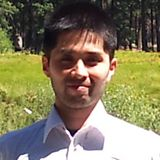
\includegraphics[height=3\baselineskip]{Tsurusawa}&
		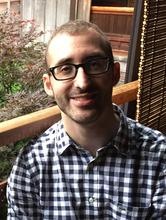
\includegraphics[height=3\baselineskip]{John}&
		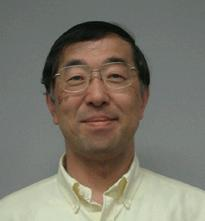
\includegraphics[height=3\baselineskip]{Tanaka}\\
		Hideyo Tsurusawa & John Russo & Hajime Tanaka\\
		U. Tokyo & U. Bristol & U. Tokyo\\
	\end{tabu}
	
	%\vfill
	%\includegraphics[height=2\baselineskip]{logo_ens-lyon}\quad
	%\includegraphics[height=2\baselineskip]{logo_ums_grand}\quad
	%\includegraphics[height=2\baselineskip]{../../Yaourt/CNRSfilaire-Q}\quad
	%\includegraphics[height=2\baselineskip]{CRPP}\quad
	%\includegraphics[height=2\baselineskip,clip=true, trim=6mm 14mm 6mm 0]{NEW-Logo-ERC-OUTLINE}
	}


\newlength{\mylength}

%\includeonly{creep_beamer}

\begin{document}
\tikzset{every mark/.append style={scale=0.8}}
\pgfplotsset{every axis/.append style={footnotesize}}

\pgfplotscreateplotcyclelist{earthy}{%
{red!40!black,mark=o},
{red!60!black,mark=triangle, every mark/.append style={rotate=180}},
{red!80!black,mark=square},
{red,mark=triangle},
{red!80!yellow, mark=diamond},
red!60!yellow,
red!40!yellow,
}

\AtBeginSection[]{
	\addtocounter{framenumber}{-1}
	\begin{frame}[plain]
		\tableofcontents[currentsection, hideothersubsections]
	\end{frame}
}

\begin{frame}{\pgfuseimage{cnrs-logo}\hspace*{0.3cm}\pgfuseimage{ucbl-logo}}%[plain]
	\titlepage
\end{frame}

\setcounter{framenumber}{0}

\begin{frame}{Crystallisation}
	\tikzsetnextfilename{whyx}%
	\begin{tikzpicture}
\node[text width=0.25\textwidth, anchor=base west] (process){
Crystallisation
\begin{itemize}
\item nucleation
\item growth
\end{itemize}};

\node[anchor=base east] (prop) at (\textwidth,0){
Properties
};

\node[text width=0.39\textwidth, anchor=base] (x) at ($(process.base east)!0.5!(prop.base west)$){
Crystalites
\begin{itemize}
\item polymorph type
\item shape
\item spatial arrangement
\item size distribution
\end{itemize}};


% 
\node[above left=3em and 0 of prop.east] (np){natural processes};
\node[below left=8em and 0 of prop.east] (tech){technological applications};

\begin{scope}[->,ultra thick, ilmcolor]
\draw (process.base east) +(0,0.3em) -- ($(x.base west)+(0,0.3em)$);
\draw (x.base) +(0,0.3em) -- ($(prop.base west)+(0,0.3em)$);
\draw (prop) -- (np.south-|prop);
\draw (prop) -- (tech.north-|prop);
\end{scope}
\end{tikzpicture}
	
	\begin{block}{Nucleation}
	\begin{itemize}
		\item 10-1000 molecules $\rightarrow$ difficult to observe
		\item classical nucleation theory (CNT): fluid $\xrightarrow{\text{1 step}}$ crystal
	\end{itemize}
	\end{block}
\end{frame}
	
\begin{frame}{Let it snow!}
	\hfill Wegener-\alert{Bergeron}-Findeisen \alert{process}
	\begin{columns}[b]
	\column{0.4\textwidth}
	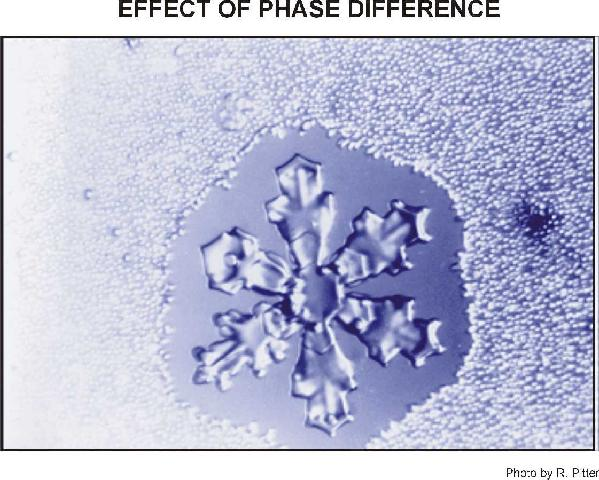
\includegraphics[width=\textwidth,clip=true,trim=0 0 0 1cm]{Pitter1.jpg}
	
	\vspace{1em}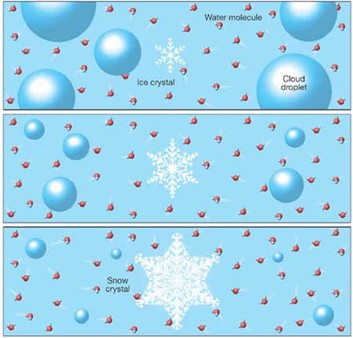
\includegraphics[width=\textwidth]{bergeron.jpg}
	\column{0.40\textwidth}
	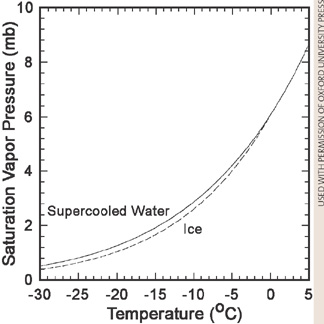
\includegraphics[width=\textwidth,clip=true,trim=0 0 0.8mm 0]{queries-figure-1.jpg}
	
	\vspace{1em}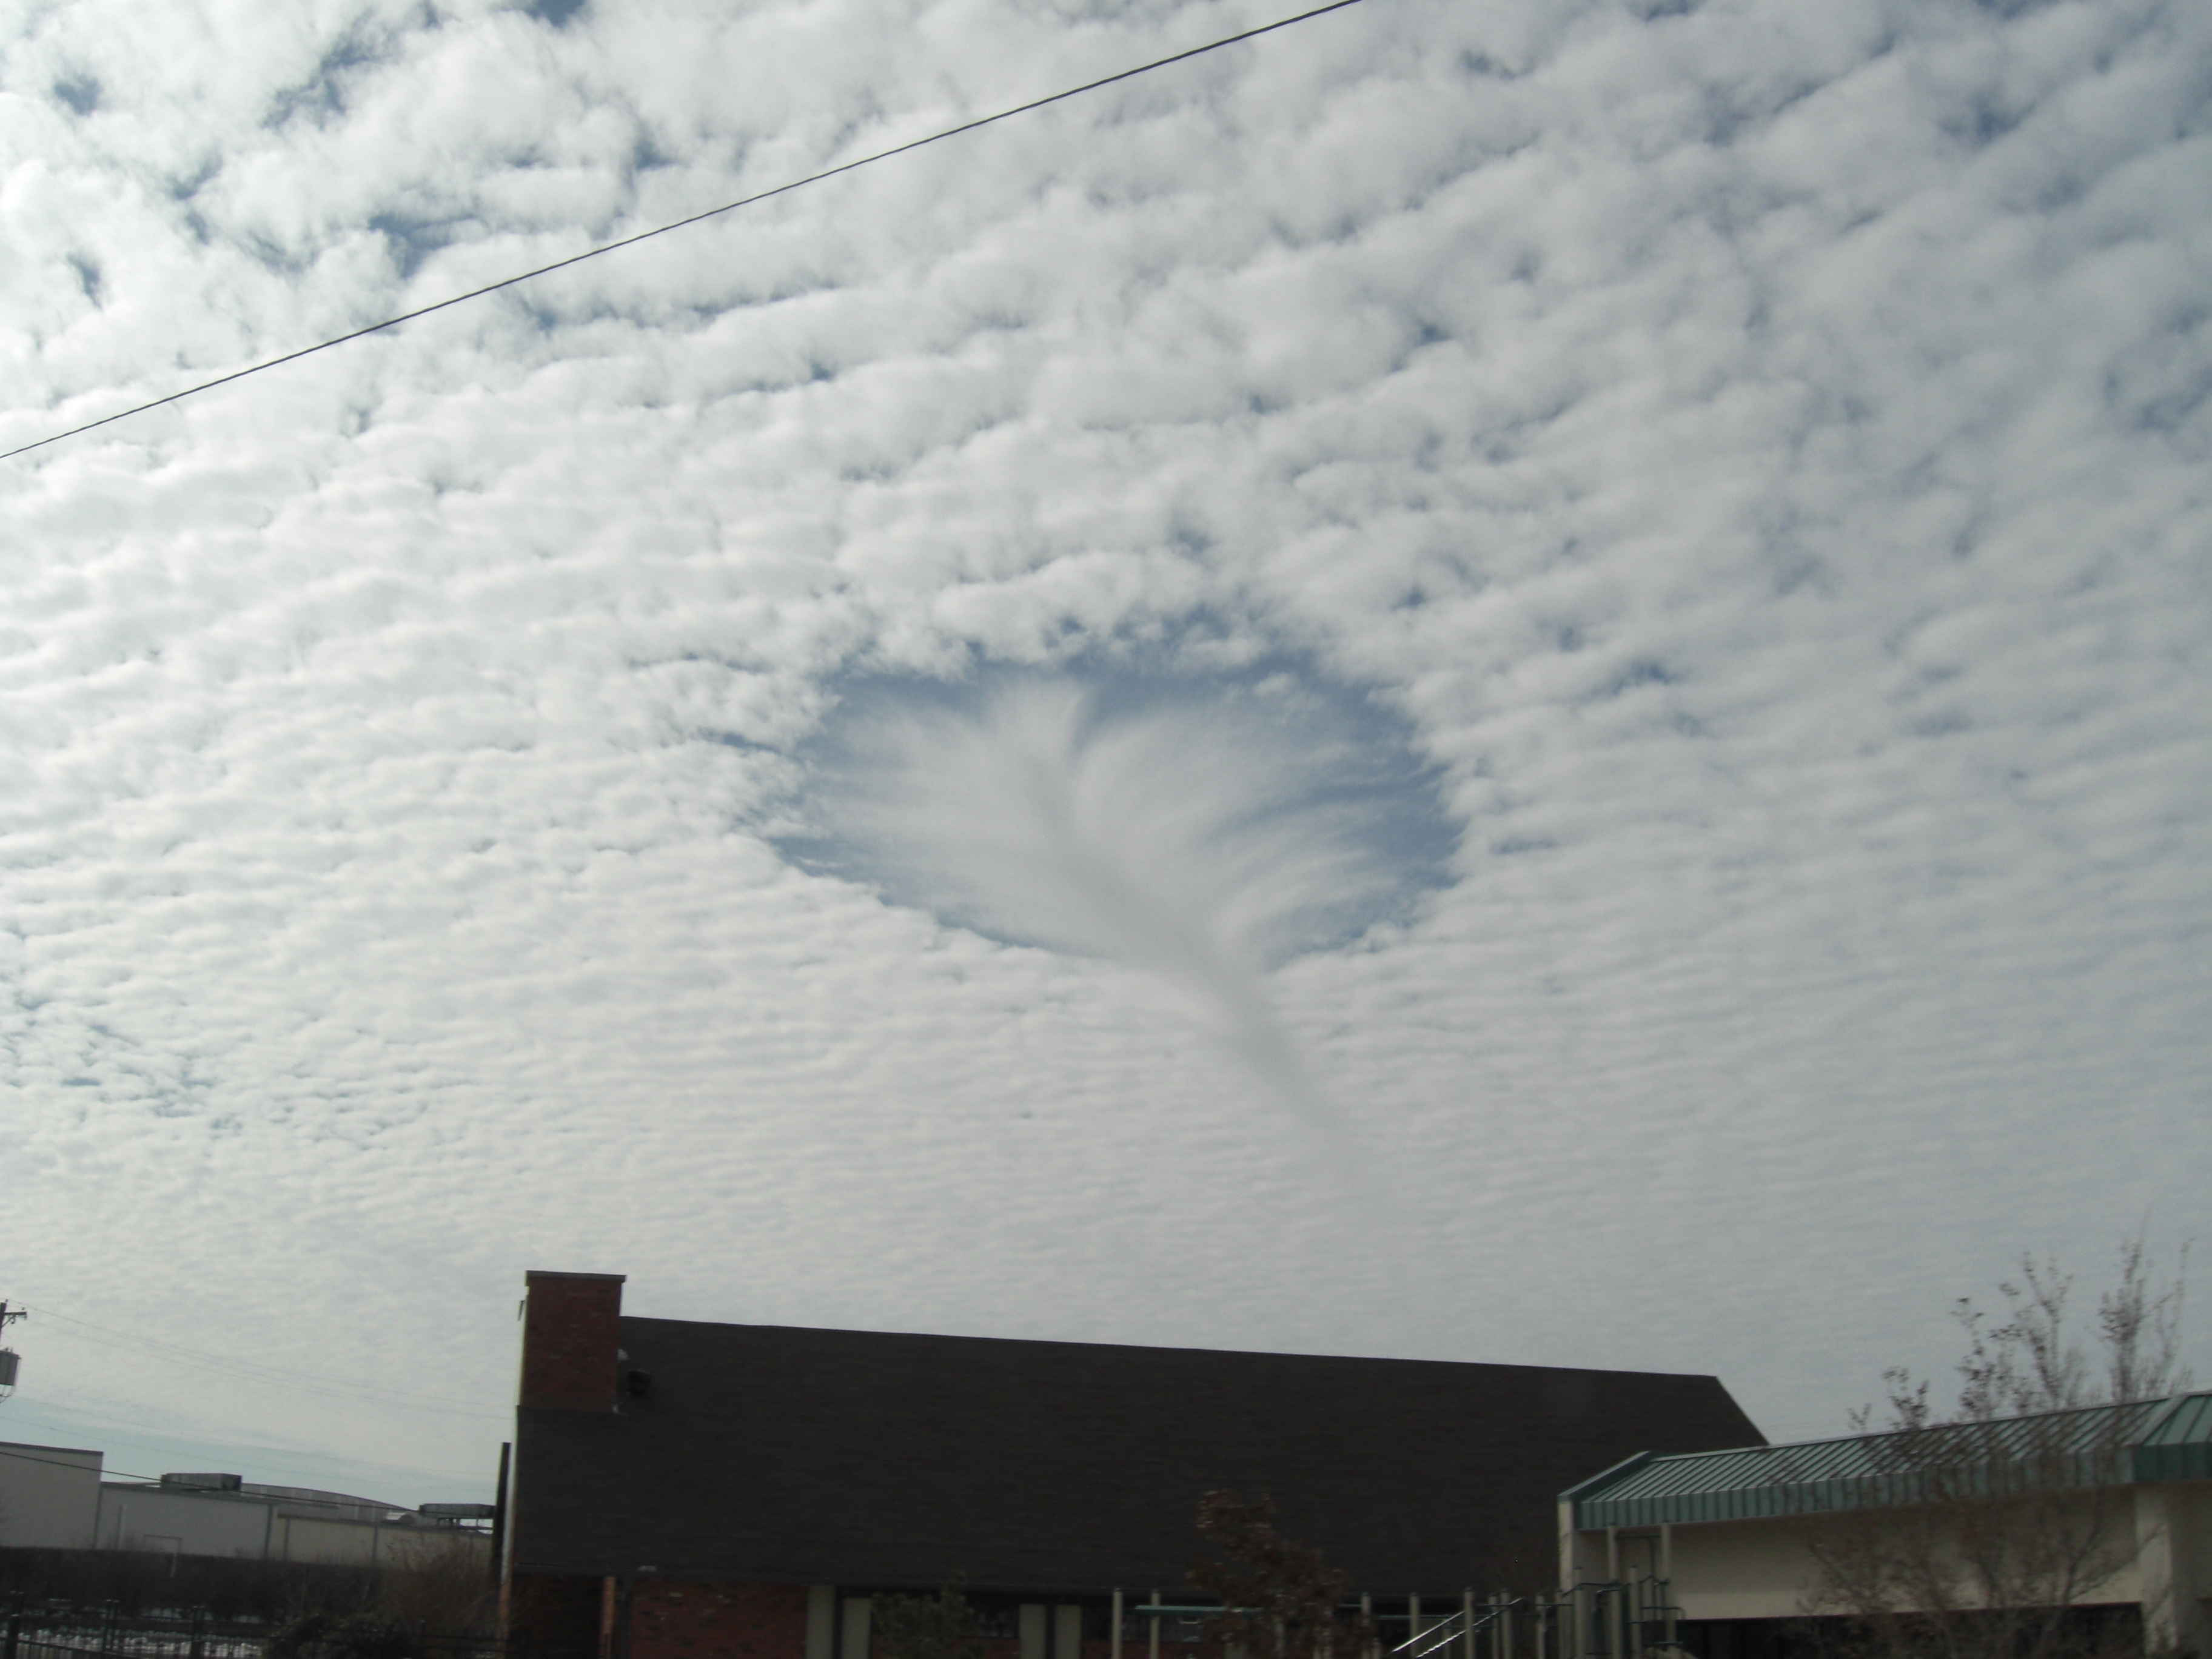
\includegraphics[width=\textwidth]{OKC-Fallstreak.jpg}
	\end{columns}
\end{frame}


\begin{frame}{Colloid + Polymer}
	
\begin{columns}
	\column{0.45\textwidth}
	\begin{tikzpicture}
		\let\mrad\relax
		\newlength\mrad
		\setlength{\mrad}{1em}
		
		
		%schemas interactions
		
		%repulsion
		\begin{scope}[xshift=2\mrad]
		\node[circle, inner sep=0, minimum width=4\mrad, inner color=Main, outer color=white]  (puri) {}; 
		\foreach \x in {0,30,...,330}{
			\draw[decoration={random steps,segment length=0.1\mrad, amplitude=0.08\mrad},decorate] (0,0) -- (\x:1\mrad);
		}
		\fill[gray, radius=0.8\mrad] circle;
		\foreach \x in {15,75,...,315}{
			\node[Accent2, font=\tiny] at (\x:0.6\mrad) {+};
		}
		\end{scope}
		
		%spheres collantes
		\begin{scope}[xshift=\textwidth-2.5\mrad]
		\node[draw,circle, inner sep=0, minimum width=2.5\mrad, green!50!black, dashed]  (colli) {}; 
		\draw[green!50!black, radius=1.25\mrad, dashed] (1.6\mrad,0) circle;
		\fill[gray, radius=0.8\mrad] circle;
		\fill[gray, radius=0.8\mrad] (1.6\mrad,0) circle;
		\end{scope}
		
		\path (puri) -- (colli) coordinate[midway] (m);
		
		%spheres dures
		\begin{scope}[shift=(m)]
		\node[circle, inner sep=0, minimum width=2.2\mrad, inner color=Main, outer color=white]  (duri) {}; 
		\foreach \x in {0,30,...,330}{
			\draw[decoration={random steps,segment length=0.1\mrad, amplitude=0.08\mrad},decorate] (0,0) -- (\x:1\mrad);
		}
		\fill[gray, radius=0.8\mrad] circle;
		\foreach \x in {15,75,...,315}{
			\node[Accent2, font=\tiny] at (\x:0.6\mrad) {+};
		}
		\end{scope}
		
		%fleches
		\draw[->] (puri) -- (duri) node[midway,above,font=\footnotesize]{ions};
		\draw[->] (duri) -- (colli)node[midway, above,font=\footnotesize]{PS};
		% \draw[->] (puri) -- (ps) -- (depli);
		
		
		%titres
		\node[text width=6em,anchor=base west, inner xsep=0] (pur) at (puri.west|-puri.north) {repulsion};
		
		\node[text width=6em,anchor=base, align=center] (dur) at (duri|-pur.base) {hard};
		
		\node[text width=6em, anchor=base east, inner xsep=0,xshift=1.5\mrad, align=right] (coll) at (colli.east|-pur.base) {depletion};
	\end{tikzpicture}	

	\bigskip
	\includegraphics[width=\textwidth]{../../CNRS-2015/Renth_sedim.jpg}\\
	\textit{\footnotesize Poon PRL 1999, Renth PRE 2001}
	\begin{itemize}
	\item triple coexistence
	\item various kinetic paths
	\end{itemize}

	\column{0.45\textwidth}
	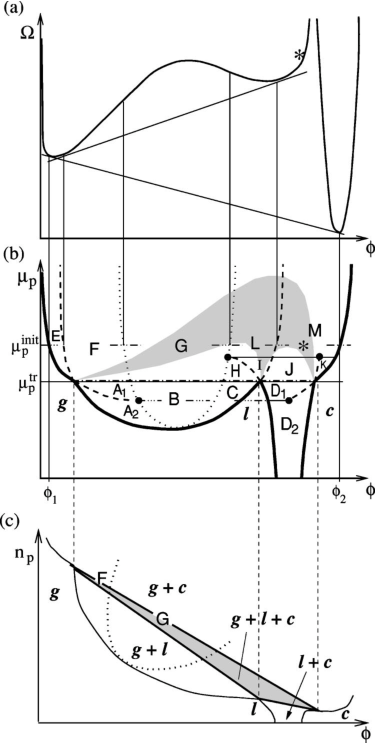
\includegraphics[width=\textwidth,clip=true,trim=0 0 0 4.5cm]{Renth_diag.pdf}
	\end{columns}
\end{frame}


\begin{frame}{Another class of gel? Crystal-gel?}
	\begin{itemize}
	\item Phase separation arrested by crystallisation
	\begin{description}
		\item[polymer blend] Tanaka \& Nishi PRL 1985
		\item[simulations] Soga J.Chem. Phys. 1999; Fortini PRE 2008 
	\end{description}
	\item Spinodal then crystallisation
	\begin{description}
		\item[simulations] Pérez Langmuir 2011
		\item[microgravity] (triple coexistence) Sabin PRL 2012
	\end{description}
	\end{itemize}
	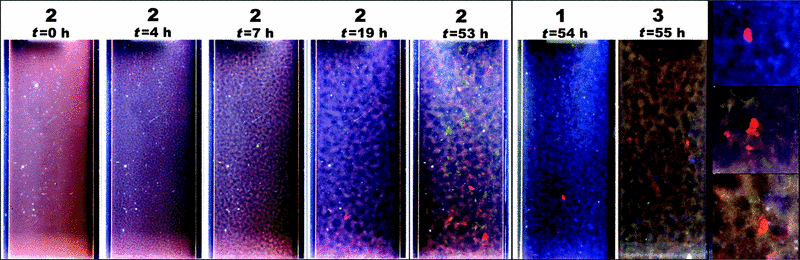
\includegraphics[width=\textwidth]{micrograv_Sabin2012}
\end{frame}

\appendix
\newcounter{finalframe}
\setcounter{finalframe}{\value{framenumber}}

\begin{frame}[plain]
\end{frame}

\setcounter{framenumber}{\value{finalframe}}
\end{document}

